\documentclass[letterpaper,twoside,10pt]{article}

\usepackage[letterpaper, margin=1in]{geometry}

\usepackage[USenglish]{babel} %francais, polish, spanish, ...
\usepackage[T1]{fontenc}
\usepackage[ansinew]{inputenc}
\usepackage{lmodern} %Type1-font for non-english texts and characters


\usepackage{graphicx} %%For loading graphic files
\usepackage{amsmath, xfrac, array, mdwlist, ulem}
\usepackage{amsthm}
\usepackage{amsfonts}
\usepackage{fancyvrb}
\usepackage[svgnames]{xcolor}
%\usepackage{natbib}
\usepackage[style=verbose, backend=bibtex]{biblatex}
\usepackage{enumitem}
\usepackage{booktabs}


\usepackage{hyperref}



\setlength{\parskip}{7pt}%
\setlength{\parindent}{0pt}%


\definecolor{LightGray}{gray}{0.9}

\bibliography{power_manual}


\makeatletter
\newif\ifFV@bgcolor
\newbox\FV@bgbox
\define@key{FV}{bgcolor}{\FV@bgcolortrue\def\FV@bgcolor{#1}}
\define@key{FV}{framecolor}{\FV@bgcolortrue\def\FV@framecolor{#1}}
\def\FV@framecolor{white}

\def\FV@BeginVBox{%
  \leavevmode\ifFV@bgcolor\setbox\FV@bgbox=\fi
  \hbox\ifx\FV@boxwidth\relax\else to\FV@boxwidth\fi\bgroup
  \ifcase\FV@baseline\vbox\or\vtop\or$\vcenter\fi\bgroup}
\def\FV@EndVBox{\egroup\ifmmode$\fi\hfil\egroup
  \ifFV@bgcolor\fcolorbox{\FV@framecolor}{\FV@bgcolor}{\box\FV@bgbox}\fi}
\makeatother

%\def\algorithmautorefname{Algorithm}


\begin{document}

\renewcommand*{\chapterautorefname}{Chapter}
\renewcommand*{\sectionautorefname}{Section}
\renewcommand*{\subsectionautorefname}{Section}
\renewcommand*{\subsubsectionautorefname}{Section}

\title{Power Estimation for VTR}
\author{Jeffrey Goeders}
%\date{} %%If commented, the current date is used.
\maketitle

The latest version of this document can be obtained here: \url{http://vtr-verilog-to-routing.googlecode.com/svn/trunk/doc/power/power_manual.pdf}

\setcounter{tocdepth}{2}
\tableofcontents %Table of contents


\newpage
\section{Overview}
This document describes the power estimation tool for VTR.  This tool provides transistor-level dynamic and static power estimates for a given architecture and circuit.

\autoref{fig:flow} illustrates how the VTR flow is modified to add power estimation.  The actual power estimation is performed within the VPR executable; however, additional files must be provided.  In addition to the circuit and architecture files, power estimation requires files detailing the signal activities and technology properties.  

\autoref{sec:running} details how to run power estimation for VTR.  \autoref{sec:tools} provides details on the supporting tools that are used to generate the signal activities and technology properties files.  \autoref{sec:arch_modelling} provides details about how the tool models architectures, including different options of modelling methods.  \autoref{sec:options} provides more advanced configuration options.

\begin{figure}[ht]
	\centering
	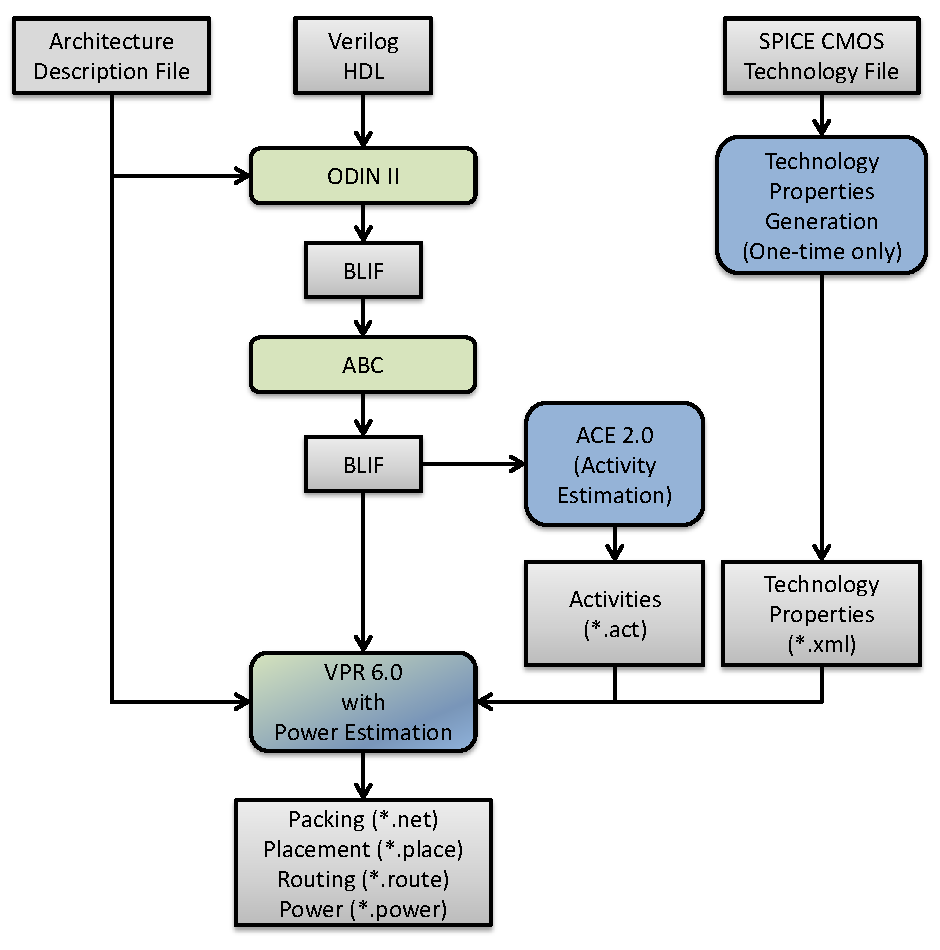
\includegraphics[scale=0.8]{images/flow.pdf}
	\caption{Power Estimation in the VTR Flow}
	\label{fig:flow}
\end{figure}


\newpage
\section{Running VTR with Power Estimation} \label{sec:running}
\subsection{VTR Flow}
	The easiest way to run the VTR flow is to use the \texttt{run\_vtr\_flow.pl} script.  See \url{http://code.google.com/p/vtr-verilog-to-routing/wiki/Run_VTR_Flow} for instructions on how to use the script.
	
In order to perform power estimation, you must add the following options:

\begin{BVerbatim}[bgcolor=LightGray, boxwidth=\textwidth]
-power 
-cmos_tech <cmos_technology_properties_file.xml>
\end{BVerbatim}	

The CMOS technology properties file is an XML file that contains relevant process-dependent information needed for power estimation. XML files for 22\,nm, 45\,nm, and 130\,nm PTM models can be found here:

\begin{BVerbatim}[bgcolor=LightGray, boxwidth=\textwidth]
<vtr>/vtr_flow/tech/.../*.xml
\end{BVerbatim}

See \autoref{sec:tpg} for information on how to generate an XML file for your own SPICE technology model.

%\subsection{VTR Tasks}
\subsection{VPR 6.0}
The easiest way to perform power estimation is to use the \texttt{run\_vtr\_flow.pl} script.  However, if you wish, you may run VPR directly.
The following command-line options are added to the VPR executable to facilitate power estimation (all are required): \newline
\texttt{\--\--power}:  Use this option to enable power estimation. \newline
\texttt{\--\--activity\_file <activities.act>}: The activity file, produce by ACE 2.0, or another tool. \newline
\texttt{\--\--tech\_properties <tech\_properties.xml>}: The technology properties XML file.

This requires a activity file, which can be generated as described in \autoref{sec:ace}.

\newpage
\section{Supporting Tools} \label{sec:tools}
\subsection{Technology Properties Generation} \label{sec:tpg}
Power estimation requires information detailing the properties of the CMOS technology.  
This information, which includes transistor capacitances, leakage currents, etc. is included in an \texttt{.xml} file, and provided as a parameter to VPR.
This XML file is generated using a script which automatically runs HSPICE, performs multiple circuit simulations, and extract the necessary values.


Some of these technology XML files are included with the release, and are located here: 

\begin{BVerbatim}[bgcolor=LightGray, boxwidth=\textwidth]
<vtr>/vtr_flow/tech/*
\end{BVerbatim}
			
If the user wishes to use a different CMOS technology file, they must run the following script.  HSPICE must be included in the \$PATH\$.

\begin{BVerbatim}[bgcolor=LightGray, boxwidth=\textwidth] 
<vtr>/vtr_flow/scripts/generate_cmos_tech_data.pl <tech_file> <tech_size> <Vdd> <temp>
\end{BVerbatim}

\texttt{<tech\_file>}: A SPICE technology file, containing a \texttt{pmos} and \texttt{nmos} models. \newline
\texttt{<tech\_size>}: The technology size, in meters. For example, a 90nm technology would have the value \texttt{90e-9}. \newline
\texttt{<Vdd>}: Supply voltage in Volts. \newline
\texttt{<temp>}: Operating temperature, in Celcius. 

\subsection{ACE 2.0 Activity Estimation} \label{sec:ace}
Power estimation requires activity information for the entire netlist.  This ativity information consists of two values:
\vspace{-10pt}
\begin{enumerate}
	\item  \underline{The Signal Probability}, $P_1$, is the long-term probability that a signal is logic-high.  For example, a clock signal with a 50\% duty cycle will have $P_1(clk) = 0.5$.
	\item \underline{The Transition Density} (or switching activity), $A_S$, is the average number of times the signal will switch during each clock cycle.  For example, a clock has $A_S(clk)=2$.
\end{enumerate}

The default tool used to perform activity estimation in VTR is ACE 2.0 \footnote{\cite{ace2}}.  
This tool was originally designed to work with the Berkeley SIS tool, which is now obsolte.  ACE 2.0 was modifed to use ABC, and is included in the VTR package here:

\begin{BVerbatim}[bgcolor=LightGray, boxwidth=\textwidth] 
<vtr>/ace2
\end{BVerbatim}

The tool can be run using the following command-line arguments:

\begin{BVerbatim}[bgcolor=LightGray, boxwidth=\textwidth] 
<vtr>/ace2/ace -b <abc.blif> -o <activities.act> -n <new.blif>
\end{BVerbatim}

\texttt{<abc.blif>}: The input BLIF file produced by ABC. \newline
\texttt{<activities.act>}: The activity file to be created. \newline
\texttt{<new.blif>}: The new BLIF file.  This will be identical in function to the ABC blif; however, since ABC does not maintain internal node names, a new BLIF must be produced with node names that match the activity file. \newline
	
User's may with to use their own activity estimation tool.  The produced activity file must contain one line for each net in the BLIF file, in the following format: 

\begin{BVerbatim}[bgcolor=LightGray, boxwidth=\textwidth] 
<net name> <signal probability> <transistion density>
\end{BVerbatim}
	

\newpage
\section{Architecture Modelling} \label{sec:arch_modelling}
The following section describes the architectural assumptions made by the power model, and the related parameters in the architecture file.

\subsection{Complex Blocks} \label{sec:clbs}
The VTR architecture description language supports a hierarchichal description of blocks.  In the architecture file, each block is described as a \texttt{pb\_type}, which may includes one or more children of type \texttt{pb\_type}, and interconnect structures to connect them.  The power estimation algorithm traverses this hierarchy recursively, and performs power estimation for each \texttt{pb\_type}.  The power model supports multiple power estimation methods, and the user specifies the desired method in the architecture file: \newline
\begin{BVerbatim}[bgcolor=LightGray, boxwidth=\textwidth] 
<pb_type>
	<power method="<est-method>">
</pb_type>
\end{BVerbatim}

The following is a list of valid estimation methods. Detailed descriptions of each type are provided in the following sections.  The methods are listed in order from most accurate to least accurate. 
\begin{enumerate}
\item \texttt{specify-size}: Detailed transistor level modelleling. The user supplies all buffer sizes and wire-lengths.  Any not provided by the user are ignored. 
\item \texttt{auto-size}: Detailed transistor level modelleling. The user can supply buffer sizes and wire-lengths; however, they will be automatically inserted when not provided. 
\item \texttt{pin-toggle}: Higher-level modelling.  The user specifies energy per toggle of the pins.  Static power provided as an absolute.
\item \texttt{C-internal}: Higher-level modelling.  The user supplies the internal capacitance of the block.  Static power provided as an absolute.
\item \texttt{absolute}: Highest-level modelling.  The user supplies both dynamic and static power as absolutes.
\end{enumerate}
Other methods of estimation:
\begin{enumerate}[resume]
\item \texttt{ignore}: The power of the \texttt{pb\_type} is ignored, including any children.
\item \texttt{sum-of-children}: Power of \texttt{pb\_type} is solely the sum of all children \texttt{pb\_types}; interconnect between the \texttt{pb\_type} and its children is ignored.
\end{enumerate}

If no estimation method is provided, it is inherited from the parent \texttt{pb\_type}. \textit{\textbf{If the top-level \texttt{pb\_type} has no estimation method, \texttt{auto-size} is assumed.}}  

\subsubsection{\texttt{specify-size}}
This estimation method provides a detailed transistor level modelling of CLBs, and will provide the most accurate power estimations.  For each \texttt{pb\_type}, power estimation accounts for the following components (See \autoref{fig:sample_clb}).
\begin{itemize*}
	\item Interconnect multiplexers
	\item Buffers and wire capacitances
	\item Child \texttt{pb\_types}
\end{itemize*}

\begin{figure}[ht]
	\centering
		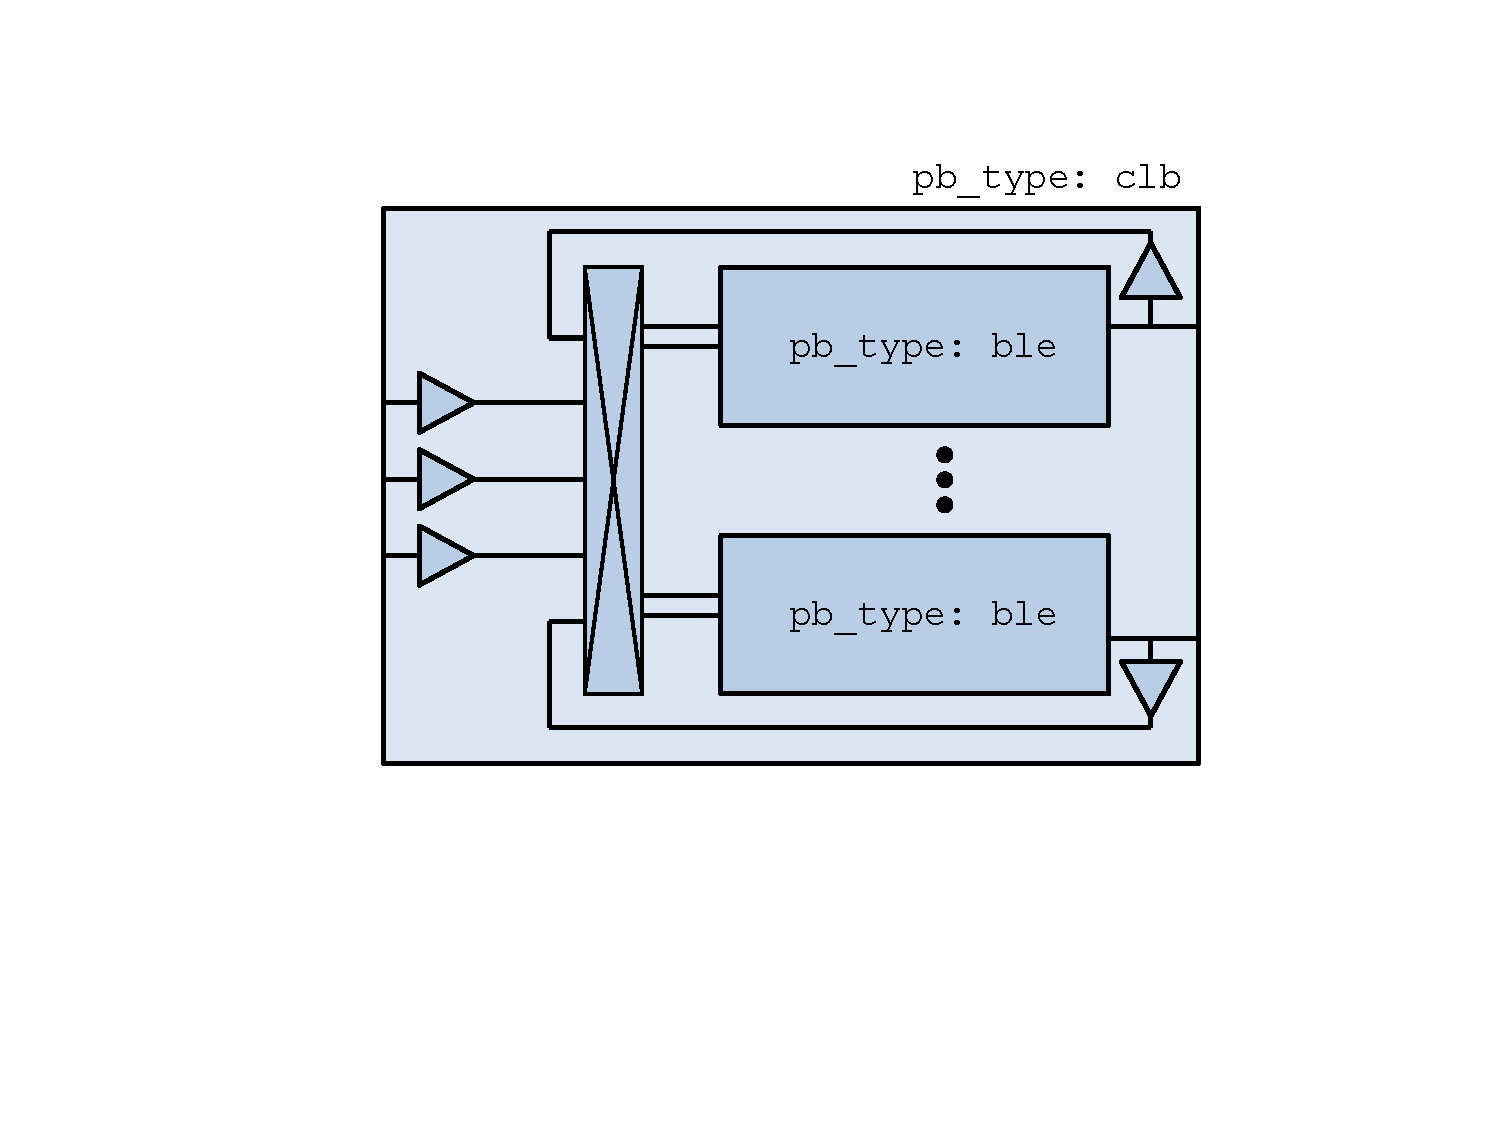
\includegraphics[scale=0.5]{images/sample_clb.pdf}
	\caption{Sample Block}
	\label{fig:sample_clb}
\end{figure}


\textbf{Multiplexers} Interconnect multiplexers are modelled as 2-level pass-transistor multiplexers, comprised of minimum-size NMOS transistors. Their size is determined automatically from the \texttt{<interconnect/>} structures in the architecture description file.  

\textbf{Buffers and Wires} Buffers and wire capacitances are not defined in the architecture file, and must be explicitly added by the user.  They are assigned on a per port basis using the following construct:

\begin{BVerbatim}[bgcolor=LightGray, boxwidth=\textwidth] 
<pb_type>
	<input name="my_input" num_pins="1">
		<power ...options.../>
	</input>
</pb_type>
\end{BVerbatim}

The wire and buffer attributes can be set using the following options.  If no options are set, it is assumed that the wire capacitance is zero, and there are no buffers present.  Keep in mind that the port construct allows for multiple pins per port.  These attributes will be applied to each pin in the port.  If necessary, the user can seperate a port into multiple ports with different wire/buffer properties.
\begin{itemize}
	\item \texttt{wire\_capacitance="1.0e-15"}: The absolute capacitance of the wire, in Farads.
	\item \texttt{wire\_length="1.0e-7"}: The absolute length of the wire, in meters.  The local interconnect capacitance option must be specified, as described in \autoref{sec:local_interc_cap}.
	\item \texttt{wire\_length="auto"}: The wirelength is automatically sized.  See \autoref{sec:local_wire_autosize}.
	\item \texttt{buffer\_size="2.0"}: The size of the buffer at this pin.  See \autoref{sec:buffer_sizing} for more information.
	\item \texttt{buffer\_size="auto"}: The size of the buffer is automatically sized, assuming it drives the above wire capacitance and a single multiplexer.  
	See \autoref{sec:buffer_sizing} for more information.
\end{itemize}

\textbf{Primitives}
For all child \texttt{pb\_types}, the algorithm performs a recursive call. Eventually \texttt{pb\_types} will be reached that have no children.  
These are primitives, such as flip-flops, LUTs, or other hard-blocks.  The power model includes functions to perform transistor-level power estimation for flip-flops and LUTs. 
If the user wishes to use a design with other primitive types (memories, multipliers, etc), they must provide an equivalent function.  If the user makes such a function, the \texttt{power\_calc\_primitive} function should be modified to call it.  Alternatively, these blocks can be configured to use higher-level power estimation methods.

%\textbf{NOTE:} Default Leakage Mode TBD

\subsubsection{\texttt{auto-size}}
This estimation method also performs detailed transistor-level modelling.  It is almost identical to the \texttt{specify-size} method described above.  The only difference is that the local wire capacitance and buffers are automatically inserted for all pins, when necessary.  This is equivalent to using the \texttt{specify-size} method with the \texttt{wire\_length="auto"} and 
\texttt{buffer\_size="auto"} options for every port.

\textbf{This is the default power estimation method.}  Although not as accurate as user-provided buffer and wire sizes, it is capable of automatically capturing trends in power dissipation as architectures are modified.  

\subsubsection{\texttt{pin-toggle}}
This method allows users to specify the dynamic power of a block in terms of the energy per toggle (in Joules) of each input, output or clock pin for the \texttt{pb\_type}.  The static power is provided as an absolute (in Watts). This is done using the following construct:

\begin{BVerbatim}[bgcolor=LightGray, boxwidth=\textwidth] 
<pb_type>	
	...
	<power method="pin-toggle">
		<port name="A" energy_per_toggle="1.0e-12"/>
		<port name="B[3:2]" energy_per_toggle="1.0e-12"/>
		<port name="C" energy_per_toggle="1.0e-12" scaled_by_static_prob="en1"/>
		<port name="D" energy_per_toggle="1.0e-12" scaled_by_static_prob_n="en2"/>
		<static_power power_per_instance="1.0e-6"/>
	</power>
</pb_type>
\end{BVerbatim}

Keep in mind that the port construct allows for multiple pins per port.  Unless an subset index is provided, the energy per toggle will be applied to each pin in the port.  The energy per toggle can be scaled by another signal using the \texttt{scaled\_by\_static\_prob}.  For example, you could scale the energy of a memory block by the read enable pin.  If the read enable were high 80\% of the time, then the energy would be scaled by the $signal\_probability$, 0.8.  Alternatively \texttt{scaled\_by\_static\_prob\_n} can be used for active low signals, and the energy will be scaled by $(1-signal\_probability)$.


This method does not perform any transistor-level estimations; the entire power estimation is performed using the above values.  It is assumed that the power usage specified here includes power of all child \texttt{pb\_types}.  No further recursive power estimation will be performed.

\subsubsection{\texttt{C-internal}}
This method allows the users to specify the dynamic power of a block in terms of the internal capacitance of the block.  The activity will be averaged across all of the input pins, and will be supplied with the internal capacitance to the standard equation $P_{dyn}=\sfrac{1}{2}\alpha CV^2$.  Again, the static power is provided as an absolute (in Watts).  This is done using the following construct:

\begin{BVerbatim}[bgcolor=LightGray, boxwidth=\textwidth] 
<pb_type>
	<power method="c-internal">
		<dynamic_power C_internal="1.0e-16"/>
		<static_power power_per_instance="1.0e-6"/>
	</power>
</pb_type>
\end{BVerbatim}

It is assumed that the power usage specified here includes power of all child \texttt{pb\_types}.  No further recursive power estimation will be performed.

\subsubsection{\texttt{absolute}}
This method is the most basic power estimation method, and allows users to specify both the dynamic and static power of a block as absolute values (in Watts).  This is done using the following construct:

\begin{BVerbatim}[bgcolor=LightGray, boxwidth=\textwidth] 
<pb_type>
	<power method="absolute">
		<dynamic_power power_per_instance="1.0e-6"/>
		<static_power power_per_instance="1.0e-6"/>
	</power>
</pb_type>
\end{BVerbatim}

It is assumed that the power usage specified here includes power of all child \texttt{pb\_types}.  No further recursive power estimation will be performed.

\subsection{Global Routing}	
Global routing consists of switch boxes and input connection boxes.

\subsubsection{Switch Boxes} \label{sec:sb}
Switch boxes are modelled as the following components (\autoref{fig:sb}):
\vspace{-10pt}
\begin{enumerate*}
	\item Multiplexer 
	\item Buffer
	\item Wire capacitance
\end{enumerate*}


\begin{figure}[ht]
	\centering
		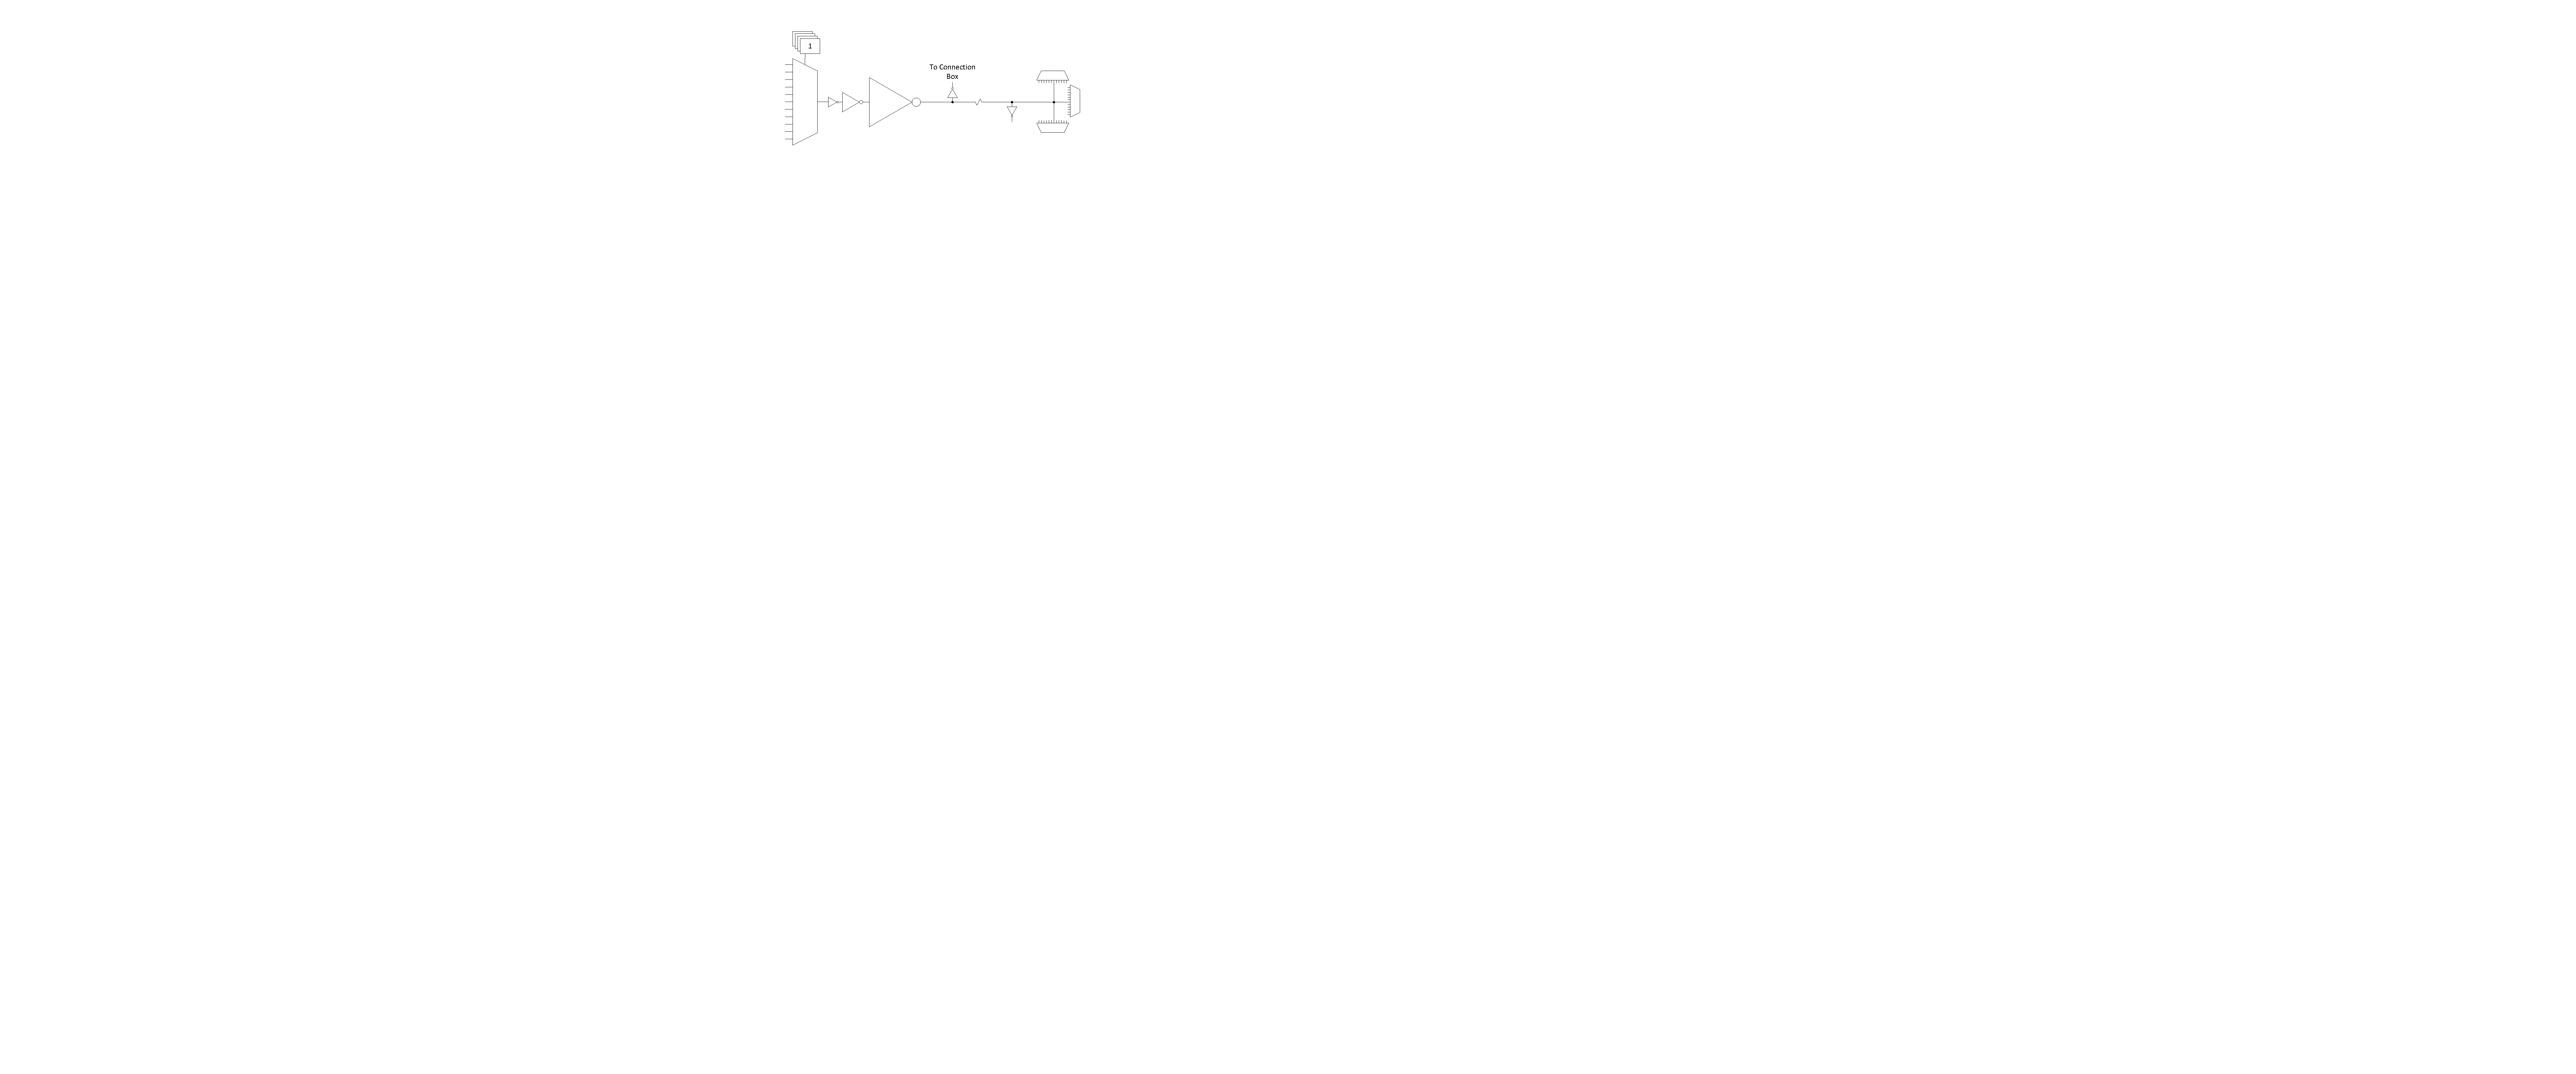
\includegraphics[scale=0.7]{images/sb.pdf}
	\caption{Switch Box}
	\label{fig:sb}
\end{figure}

\textbf{Multiplexer} 
	The multiplexer is modelled as 2-level pass-transistor multiplexer, comprised of minimum-size NMOS transistors.  
	The number of inputs to the multiplexer is automatically determined.
	
\textbf{Buffer} 
The buffer is a multistage CMOS buffer.  The buffer size is determined based upon output capacitance provided in the architecture file: 

\begin{BVerbatim}[bgcolor=LightGray, boxwidth=\textwidth] 
<switchlist>
	<switch type="mux" ... C_out="XXX"
</switchlist>
\end{BVerbatim}

The user may override this method by providing the buffer size as shown below:

\begin{BVerbatim}[bgcolor=LightGray, boxwidth=\textwidth] 
<switchlist>
	<switch type="mux" ... power_buf_size="16.0"
</switchlist>
\end{BVerbatim}

The size is the drive strength of the buffer, relative to a minimum-sized inverter.

%Alternatively, the size can be replaced by the "\texttt{auto}" keyword, and the buffer will be automatically sized based on the load capacitance.  See \autoref{sec:buffer_sizing} for information about buffer sizings. 

%\textbf{Wire Capacitance} The wire capacitance is determined using the information in the architecture file:
%
%\begin{BVerbatim}[bgcolor=LightGray, boxwidth=\textwidth] 
%<segmentlist>
%	<segment type="unidir" ... Cmetal="XXX" .../>
%</segmentlist>
%\end{BVerbatim}

%The following options can be used to specify wire capacitance:
%\vspace{-10pt}
%\begin{itemize*}
%\item \texttt{power\_wire\_c}: Absolute wire capacitance, in farads.
%\item \texttt{power\_wire\_c\_per\_m}: Wire capacitance in farads per meter.  The capacitance is calculated using an automatically determined wirelength, based on the area of a tile in the FPGA (\autoref{sec:area_est}).
%\end{itemize*}

\subsection{Input Connection Boxes} \label{sec:cb}
Input connection boxes are modelled as the following components (\autoref{fig:cb}):
\vspace{-10pt}
\begin{itemize}
\item One buffer per routing track, sized to drive the load of all input multiplexers to which the buffer is connected (For buffer sizing see \autoref{sec:buffer_sizing}).
\item One multiplexer per block input pin, sized according to the number of routing tracks that connect to the pin.
\end{itemize}

\begin{figure}[ht]
	\centering
		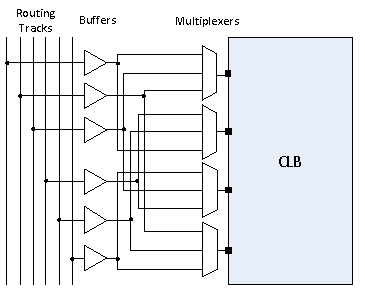
\includegraphics[scale=1.6]{images/cb.pdf}
	\caption{Conneciton Box}
	\label{fig:cb}
\end{figure}


\subsection{Clock Network}
The clock network modelled is a four quadrant spine and rib design, as illustrated in \autoref{fig:clock_network}. At this time, the power model only supports a single clock.
The model assumes that the entire spine and rib clock network will contain buffers separated in distance by the length of a grid tile.  
The buffer sizes and wire capacitances are specified in the architecture file using the following construct:

\begin{BVerbatim}[bgcolor=LightGray, boxwidth=\textwidth] 
<clocks>
	<clock ... clock_options .../>
</clocks>
\end{BVerbatim}


The following clock options are supported:
\vspace{-10pt}
\begin{itemize}
\item \texttt{C\_wire="1e-16"}: The absolute capacitance, in fards, of the wire between each clock buffer.
\item \texttt{C\_wire\_per\_m="1e-12"}: The wire capacitance, in fards per m.  The capacitance is calculated using an automatically determined wirelength, based on the area of a tile in the FPGA.
\item \texttt{buffer\_size="2.0"}: The size of each clock buffer.  This can be replaced with the "auto" keyword.  See \autoref{sec:buffer_sizing} for more information on buffer sizing.
\end{itemize}

\begin{figure}[ht]
	\centering
	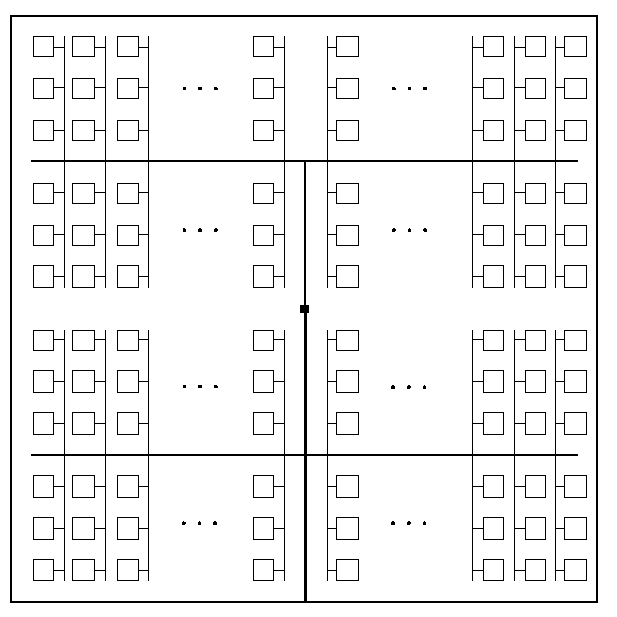
\includegraphics[scale=0.7]{images/clock_network}
	\caption{The clock network.  Squares represent CLBs, and the wires represent the clock network.}
	\label{fig:clock_network}
\end{figure}




\clearpage
\section{Other Architecture Options \& Techniques} \label{sec:options}


\subsection{Local Wire Auto-Sizing} \label{sec:local_wire_autosize}
Due to the significant user effort required to provide local buffer and wire sizes, we developed an algorithm to estimate them automatically.  
This algorithm recursively calculates the area of all entities within a CLB, which consists of the area of primitives and the area of local interconnect multiplexers.  
If an architecture uses new primitives in CLBs, it should include a function that returns the transistor count.  This function should be called from within \texttt{power\_count\_transistors\_primitive()}.


 In order to determine the wire length that connects a parent entity to its children, the following assumptions are made:

\begin{itemize}
	\item Assumption 1: All components (CLB entities, multiplexers, crossbars) are assumed to be contained in a square-shaped area.
	\item Assumption 2: All wires connecting a parent entity to its child pass through the \emph{interconnect square}, which is the sum area of all interconnect multiplexers belonging to the parent entity.
\end{itemize}
	
\autoref{fig:local_interc} provides an illustration of a parent entity connected to its child entities, containing one of each interconnect type (direct, many-to-1, and complete).  In this figure,
the square on the left represents the area used by the transistors of the interconnect multiplexers.  It is assumed that all connections from parent to child will pass through this area.  Real wire lengths could me more or less than this estimate; some pins in the parent may be directly adjacent to child entities, or they may have to 
traverse a distance greater than just the interconnect area.  Unfortuantely, a more rigorous estimation would require some information about the transistor layout.	



\begin{figure}[ht]
	\centering
	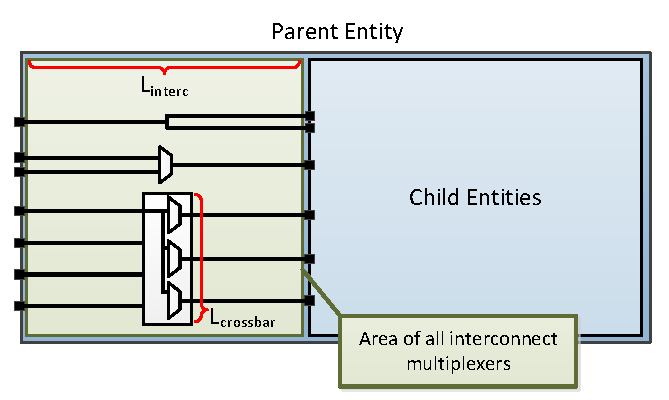
\includegraphics[width=\textwidth]{images/local_interc}
	\caption[D Flip-Flop]{Local interconnect wirelength.}
	\label{fig:local_interc}
\end{figure}

\begin{table}
		\centering
		\begin{tabular}{lccc}\toprule
		Connection from Entity Pin to:  & Estimated Wirelength & Transistor  Capacitance \\ \midrule
		Direct (Input or Output) & $0.5 \cdot L_{interc}$ & 0\\ 
		Many-to-1 (Input or Output)  & $0.5 \cdot L_{interc}$ & $C_{INV}$ \\ 
		Complete $m$:$n$ (Input) &$0.5 \cdot L_{interc} + L_{crossbar}$ & $n\cdot C_{INV}$ \\
		Complete $m$:$n$ (Output) & $0.5 \cdot L_{interc}$ & $C_{INV}$\\ \bottomrule
		\end{tabular}
	\caption{Local interconnect wirelength and capacitance.  ($C_{INV}$ is the input capacitance of a minimum-sized inverter.)}
	\label{tab:local_interc_wirelength}	
\end{table}

\autoref{tab:local_interc_wirelength} details how local wire lengths are determined as a function of entity and interconnect areas.
It is assumed that each wire connecting a pin of a \texttt{pb\_type} to an interconnect structure is of length $0.5 \cdot L_{interc}$.  In reality, this length depends on the actual transistor
layout, and may be much larger or much smaller than the estimated value.  If desired, the user can override the 0.5 constant in the architecture file:


\begin{BVerbatim}[bgcolor=LightGray, boxwidth=\textwidth] 
<architecture>
	<power>
		<local_interconnect factor="0.5">
	</power>
</architecture>
\end{BVerbatim}

\subsection{Buffer Sizing} \label{sec:buffer_sizing}
In the power estimator, a buffer size refers to the size of the final stage of multi-stage buffer (if small, only a single stage is used).  The specified size is the (\sfrac{W}{L}) of the NMOS transistor.  The PMOS transistor will automatically be sized larger.    
Generally, buffers are sized depending on the load capacitance, using the following equation:

\begin{align}
	\text{Buffer Size}=\frac{1}{2\cdot f_{LE}}*\frac{C_{Load}}{C_{INV}}
	\label{eq:autosize}
\end{align}	
In this equation, $C_{INV}$ is the input capacitance of a minimum-sized inverter, and $f_{LE}$ is the logical effort factor.  The logical effort factor is the gain between stages of the multi-stage buffer, which by default is 4 (minimal delay).  The term $(2\cdot f_{LE})$ is used so that the ratio of the final stage to the driven capacitance is smaller.  This produces a much lower-area, lower-power buffer that is still close to the optimal delay, more representative of common design practises. The logical effort factor can be modified in the architecture file: 


\begin{BVerbatim}[bgcolor=LightGray, boxwidth=\textwidth] 
<architecture>
	<power>
		<buffers logical_effort_factor="4">
	</power>
</architecture>
\end{BVerbatim}

%The number of buffer stages is chosen such that each stage is close to $f_{LE}$ times larger than the previous stage.






\subsection{Local Interconnect Capacitance} \label{sec:local_interc_cap}
If using the \texttt{auto-size} or \texttt{wire-length} options (\autoref{sec:clbs}), the local interconnect capacitance must be specified.  This is specified in the units of Farads/meter.

\begin{BVerbatim}[bgcolor=LightGray, boxwidth=\textwidth] 
<architecture>
	<power>
		<local_interconnect C_wire="2.5e-15">
	</power>
</architecture>
\end{BVerbatim}


%\subsection{SRAM}
%TBD

\newpage
\section{Support}
For support, please check \url{http://code.google.com/p/vtr-verilog-to-routing/wiki/Power}, or email \href{mailto:vtr.power.estimation@gmail.com}{vtr.power.estimation@gmail.com}.

\end{document}

